\documentclass[twocolumn,twocolappendix,trackchanges]{aastex63}
\usepackage{amsmath}
\newcommand{\code}[1]{\texttt{#1}}
\newcommand{\mesa}{\code{MESA}}
\newcommand{\MESA}{\code{MESA}}
\renewcommand{\labelitemii}{$\bullet$}
\newcommand{\kms}{{\mathrm{km\ s^{-1}}}}
\newcommand{\Msun}{{\mathrm{M}_\odot}}
\newcommand{\kev}{\mathrm{keV}}
\newcommand{\gk}{\ensuremath{\,\rm{GK}}}
\usepackage{CJK}
\DeclareRobustCommand{\Eqref}[1]{Eq.~\ref{#1}}
\DeclareRobustCommand{\Figref}[1]{Fig.~\ref{#1}}
\DeclareRobustCommand{\Tabref}[1]{Tab.~\ref{#1}}
\DeclareRobustCommand{\Secref}[1]{Sec.~\ref{#1}}
\newcommand{\zoph}{$\zeta$ Oph}

\newcommand{\todo}[1]{{\large $\blacksquare$~\textbf{\color{red}[#1]}}~$\blacksquare$}

\begin{document}

\graphicspath{{./figures/}}


\title{Testing models of accreting stars in
  massive binaries on $\zeta$ Ophiuchi}
\author[0000-0002-6718-9472]{M.~Renzo}
\affiliation{Department of Physics, Columbia University, New York, NY 10027, USA}
\affiliation{Center for Computational Astrophysics, Flatiron Institute, New York, NY 10010, USA}

\author{\todo{TBD}}

\begin{abstract}
  Binarity dominates the evolution of massive stars, and the nearest
  O-type star to Earth, $\zeta$ Ophiuchi, has long been proposed to be
  a product of binary evolution. Despite this, most stellar models
  have tried unsuccessfully to reproduce its observable properties
  relying on single-star rotating models.  \todo{Here we do better}
\end{abstract}

\vspace*{-10pt}
\keywords{stars: individual: $\zeta$ Ophiuchi  -- stars: massive --
  stars: binaries} %% check keywords exist


%% main text limit:
%% 3500 words, 50 references, 5 figures (each up to 9 panels)
\section{Introduction}
\label{sec:intro}


The nearest O-type star to Earth is $\zeta$ Ophiuchi\footnote{also known
as HD\,149\,757.} \citep[spectral
type O9.5{\rm IVnn},][]{sota:14}, at % with a parallax of
% 5-8\,milliarcsec corresponding to
a distance of $\sim$110\,pc \citep[e.g.,][and references
therein]{neuhauser:20}. It was originally identified as a runaway star
through its large proper motion by \cite{blaauw:52}.  Unfortunately,
the \emph{Gaia} data for this object are not of sufficient quality to
improve previous astrometric results, but estimates of the peculiar
velocity range in $30-50\,\kms$
\citep[e.g.,][]{zehe:18, neuhauser:20}. The
large velocity with respect the surrounding interstellar material is
also confirmed by the presence of a prominent bow-shock
\citep[e.g.,][]{bodensteiner:18}.

Because of its young apparent age, extremely fast rotation
($v\sin(i)\gtrsim 400\,\kms$, e.g., \citealt{zehe:18}), and nitrogen
(N) and helium (He) rich surface \citep[e.g.,][]{herrero:92,
  blaauw:93, villamariz:05, marcolino:09}, \zoph\ is a prime candidate
for the binary supernova scenario \citep{blaauw:61, renzo:19walk}. In
this scenario, after a phase of mass transfer in a massive binary
which can spin up the accreting star \citep[e.g.,][]{packet:81}, the
core-collapse of the donor star disrupts the binary. This results in
the ejection of the former accretor as a fast rotator and with its
pre-explosion orbital velocity as peculiar velocity.

Many studies have suggested \zoph\ might have accreted mass from a
companion before acquiring its large velocity, both from spectroscopic
and kinematic considerations \citep[e.g.,][]{blaauw:93, hoogerwerf:00,
  hoogerwerf:01, tetzlaff:10, neuhauser:20} and using stellar modeling
arguments \citep[e.g.,][]{vanrensbergen:96}. Recently,
\cite{neuhauser:20} suggested that a supernova in
Upper-Centaurus-Lupus produced the pulsar PSR B1706-16, ejected \zoph,
and also injected the short-lived radioactive isotope
$^{60}\mathrm{Fe}$ on Earth about $\sim 1.5$\,Myr ago. This argues
strongly for a successful supernova explosion accompanied by a large
$\sim 250\,\kms$ natal kick, which in most cases would be sufficient
to disrupt the binary.

Although the nature of \zoph\ as a binary product is well
established, its large rotation rate has lead most attempts to explain
the surface composition to rely on rotational mixing
\cite[e.g.,][]{maeder:00}. Even the binary models of
\cite{vanrensbergen:96} assumed spin-up due to mass accretion
\citep[e.g.,][]{packet:81} to drive rotational mixing from the
interior of the accreting star (see also
\citealt{cantiello:07}). However, \cite{villamariz:05} were unable to
find good fit for the stellar spectra using the rotating models from
\cite{meynet:00}.

This may not be surprising: rotational mixing has
lower efficiency for metal-rich and relatively low mass stars because
of the increased importance of mean molecular weight gradients and
longer thermal timescales compared to more massive stars
\citep[e.g.,][]{yoon:06, perna:14}. The parent association of $\zeta$
Oph has $Z=0.01-0.02\simeq Z_\odot$ \citep[e.g.,][]{murphy:21}, and
mass estimates for the star range from $13-25\,M_\odot$, at the
lower end of the range where efficient mixing might bring He and
CNO-processed material to the surface (chemically homogeneous
evolution).

% \todo{maybe paragraph below goes in discussion}
On top of the surface abundances, its extreme rotation rate, and the
peculiar space velocity, \zoph\ poses a number of other
puzzles: its wind mass-loss rate is about two orders of magnitude
lower than theoretical predictions (weak wind problem,
\citealt{marcolino:09}), the star exhibits spectral variability with
occasional appearance of H$\alpha$ in emission
\citep[e.g.,][]{walker:79}, and is potentially magnetic \todo{true?ref?}.

Given the challenges in explaining the surface composition of \zoph\
with rotational mixing from the stellar interior and the strong
evidence for its past as a member of a binary system, this star offers
a unique opportunity to constrain the evolution of accreting stars in
massive binary systems, which is hard to model because of the
interplay of rotation, mixing, and accretion
\citep[e.g.][]{hellings:83, hellings:84, braun:95}.

While we focus here on this particular star, we emphasize that
understanding the evolution of  accretors in massive binaries has
wider and crucial implications. Observed stellar populations might
contain $\sim10\%$ of presently single O-type that accreted mass
previously \citep{renzo:19walk}, gravitational-wave progenitors in
isolated binary formation scenarios go through a common envelope phase
initiated by the originally less massive accretor after the formation
of the first compact object \citep[e.g.,][]{belczynski:16nat, tauris:17,
  law-smith:20}, \todo{more reasons?}

Here, we present the first self-consistent binary evolution model for
$\zeta$ Oph computing simultaneously the coupled evolution of
\emph{both} donor
and accretor star. After presenting our calculations in
\Secref{sec:methods}, we show our best model which reproduces the
majority of the salient features of this star in
\Secref{sec:best_model}. In this model, the surface abundances of
\zoph\ are explained by pollution from the former companion, rather
than upward mixing from the interior of \zoph\ itself. We discuss the
sensitivity of our results to the admittedly many free parameters
required for this kind of computations in
\Secref{sec:param_variations}. Finally, we conclude in
\Secref{sec:conclusions}.

\section{Modeling mass transfer with \texttt{MESA}}
\label{sec:methods}


\todo{  Methods:
  \begin{itemize}
  \item self-consistent modeling of the evolution
  \item depends on many free parameters governing the intricate and
    coupled physics of mass transfer, mixing, rotation
  \end{itemize}
}

\section{Best model}
\label{sec:best_model}

\begin{figure}[htbp]
  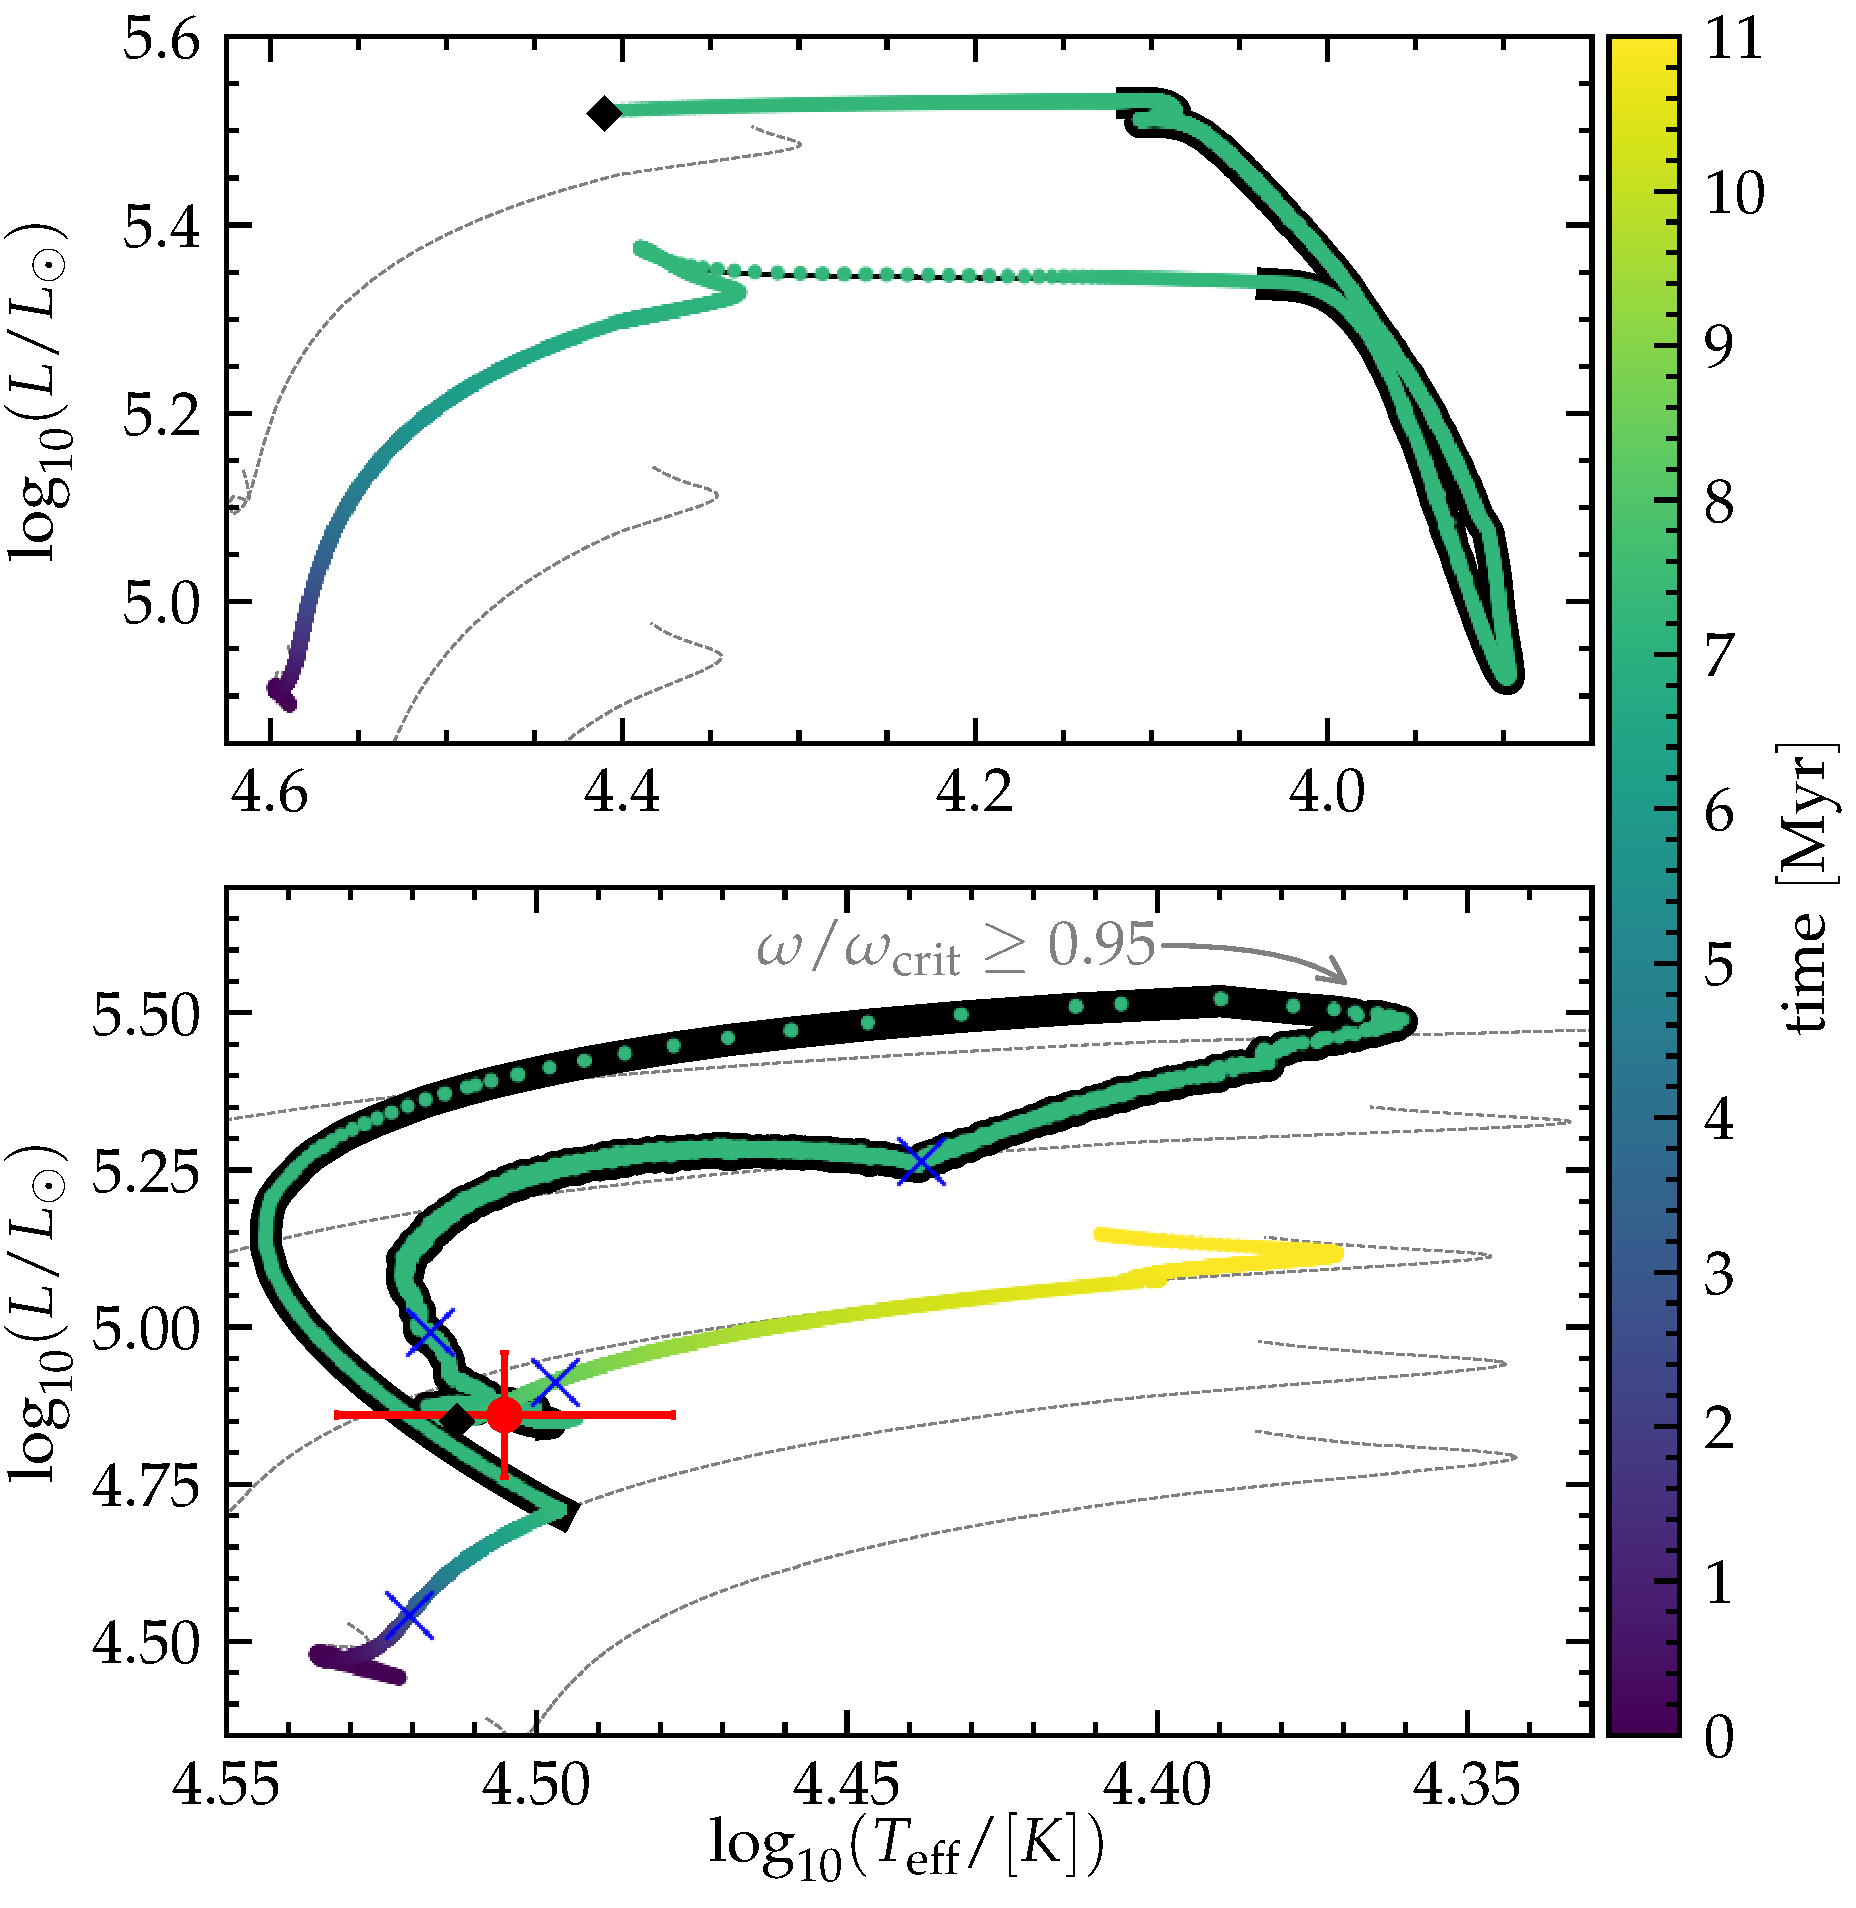
\includegraphics[width=0.5\textwidth]{HRD_both}
  \caption{Hertzsprung-Russell diagram for the progenitor binary of
    \zoph. The bottom (top) panel shows the accretor (donor), with the
    color indicating the surface $^4\mathrm{He}$ mass fraction. The
    red datapoint shows the position of \zoph\ according to
    \cite{villamariz:05}. Note the different scale on the two panels,
    and that the bottom panel shows a longer time, until the end of
    the accretor's main sequence.}
  \label{fig:HRD_both}
\end{figure}

\begin{figure}[htbp]
  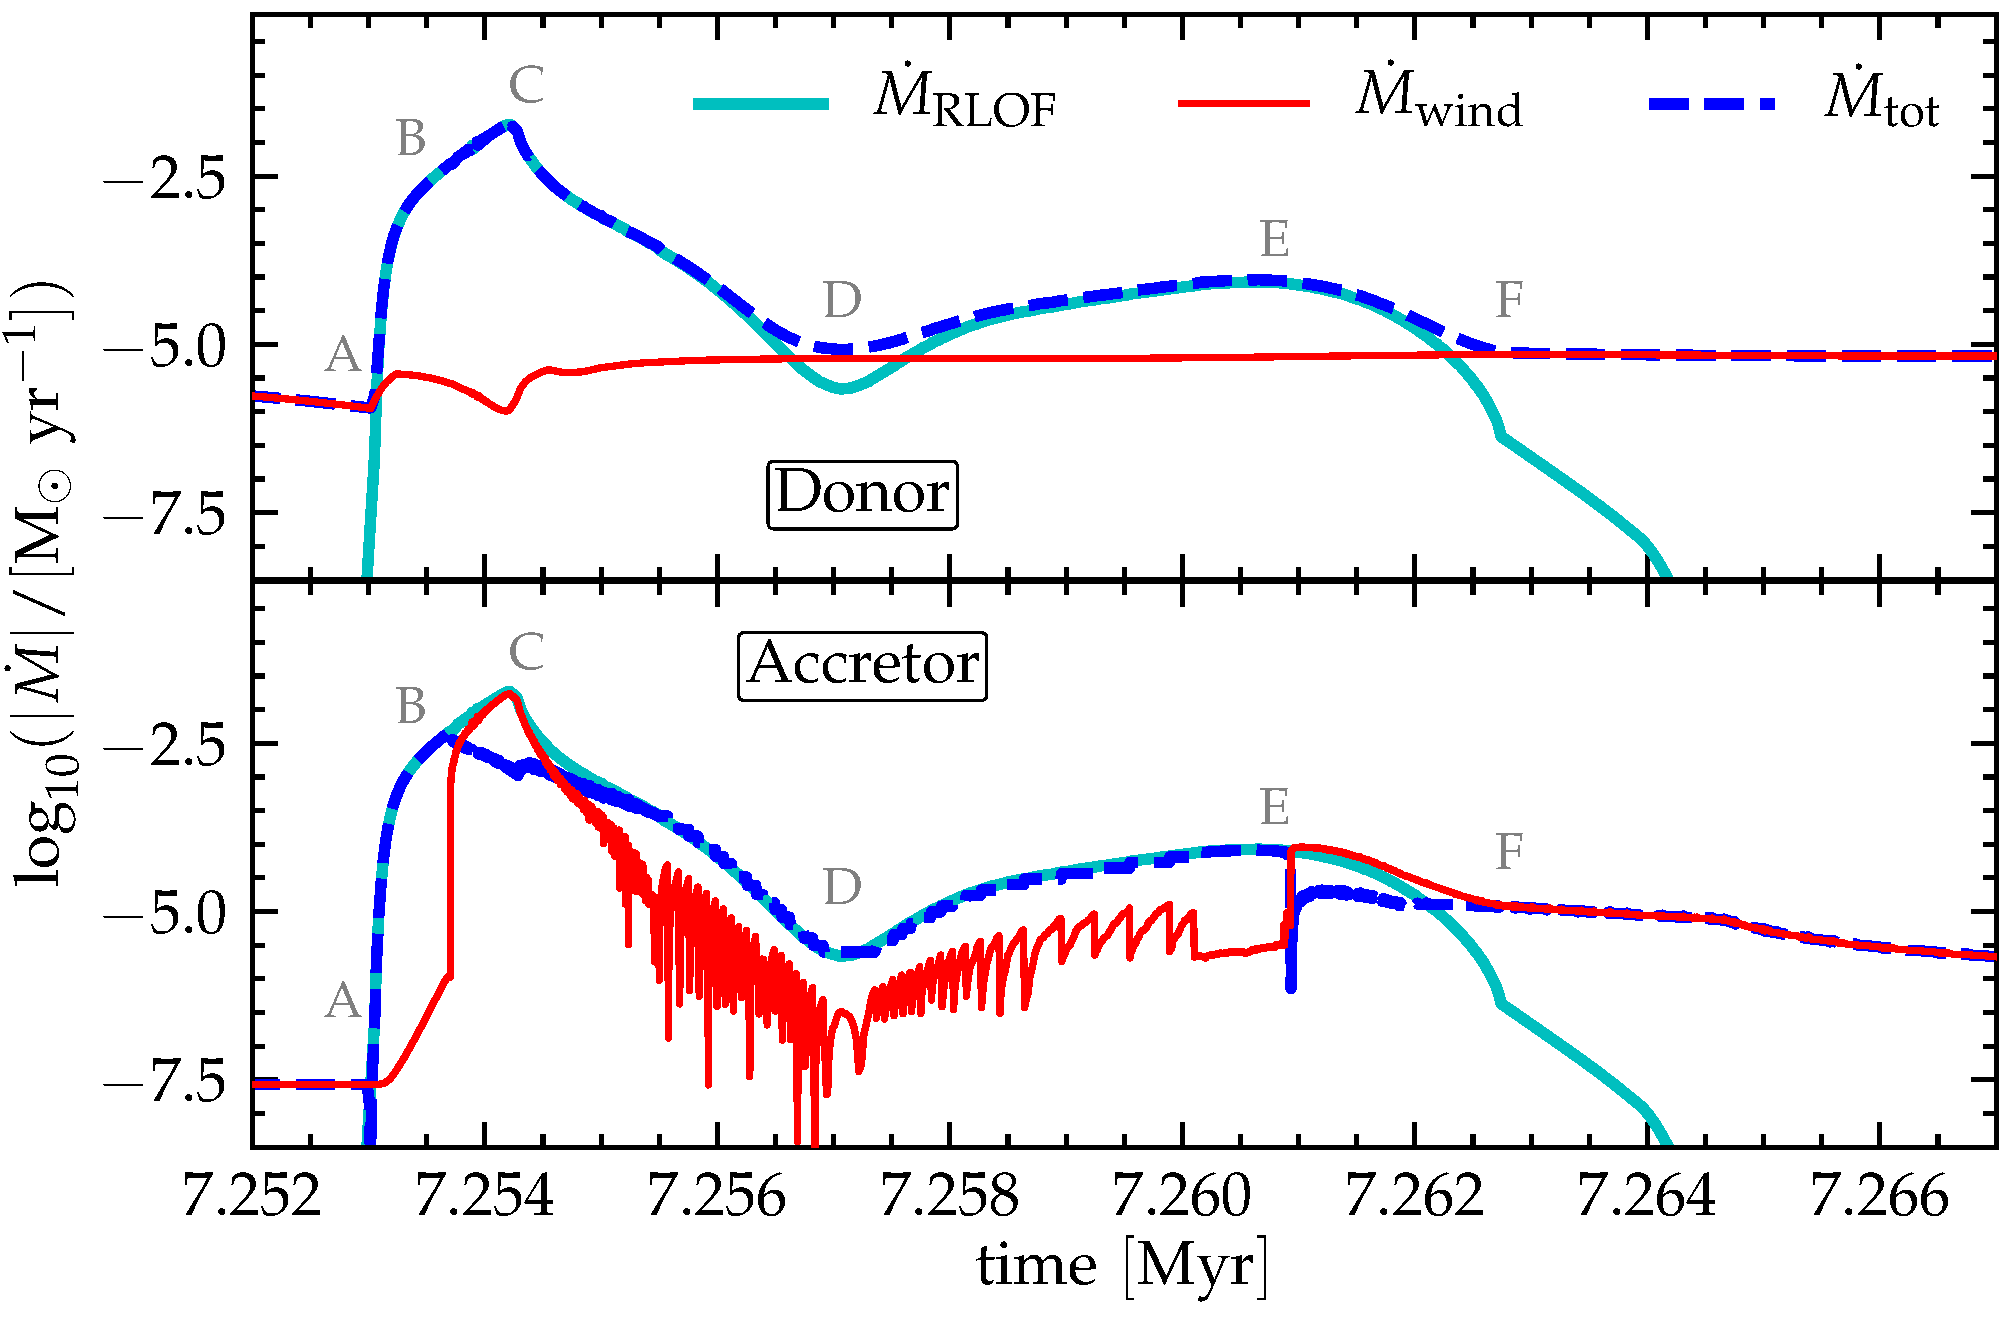
\includegraphics[width=0.5\textwidth]{MT}
  \caption{Mass transfer history during RLOF. The top (bottom) panel
    shows the donor (accretor) star. The cyan solid line shows the
    mass transfer rate between the two stars, the dashed blue line
    shows the actual change in the mass of the stars, and the thin red
    line shows the wind mass loss rates. During RLOF the accretor
    reaches critical rotation, which leads to oscillations in the
    rotationally-enhahnced wind mass loss. \todo{better x-axis}}
  \label{fig:MT}
\end{figure}

\begin{figure}[htbp]
  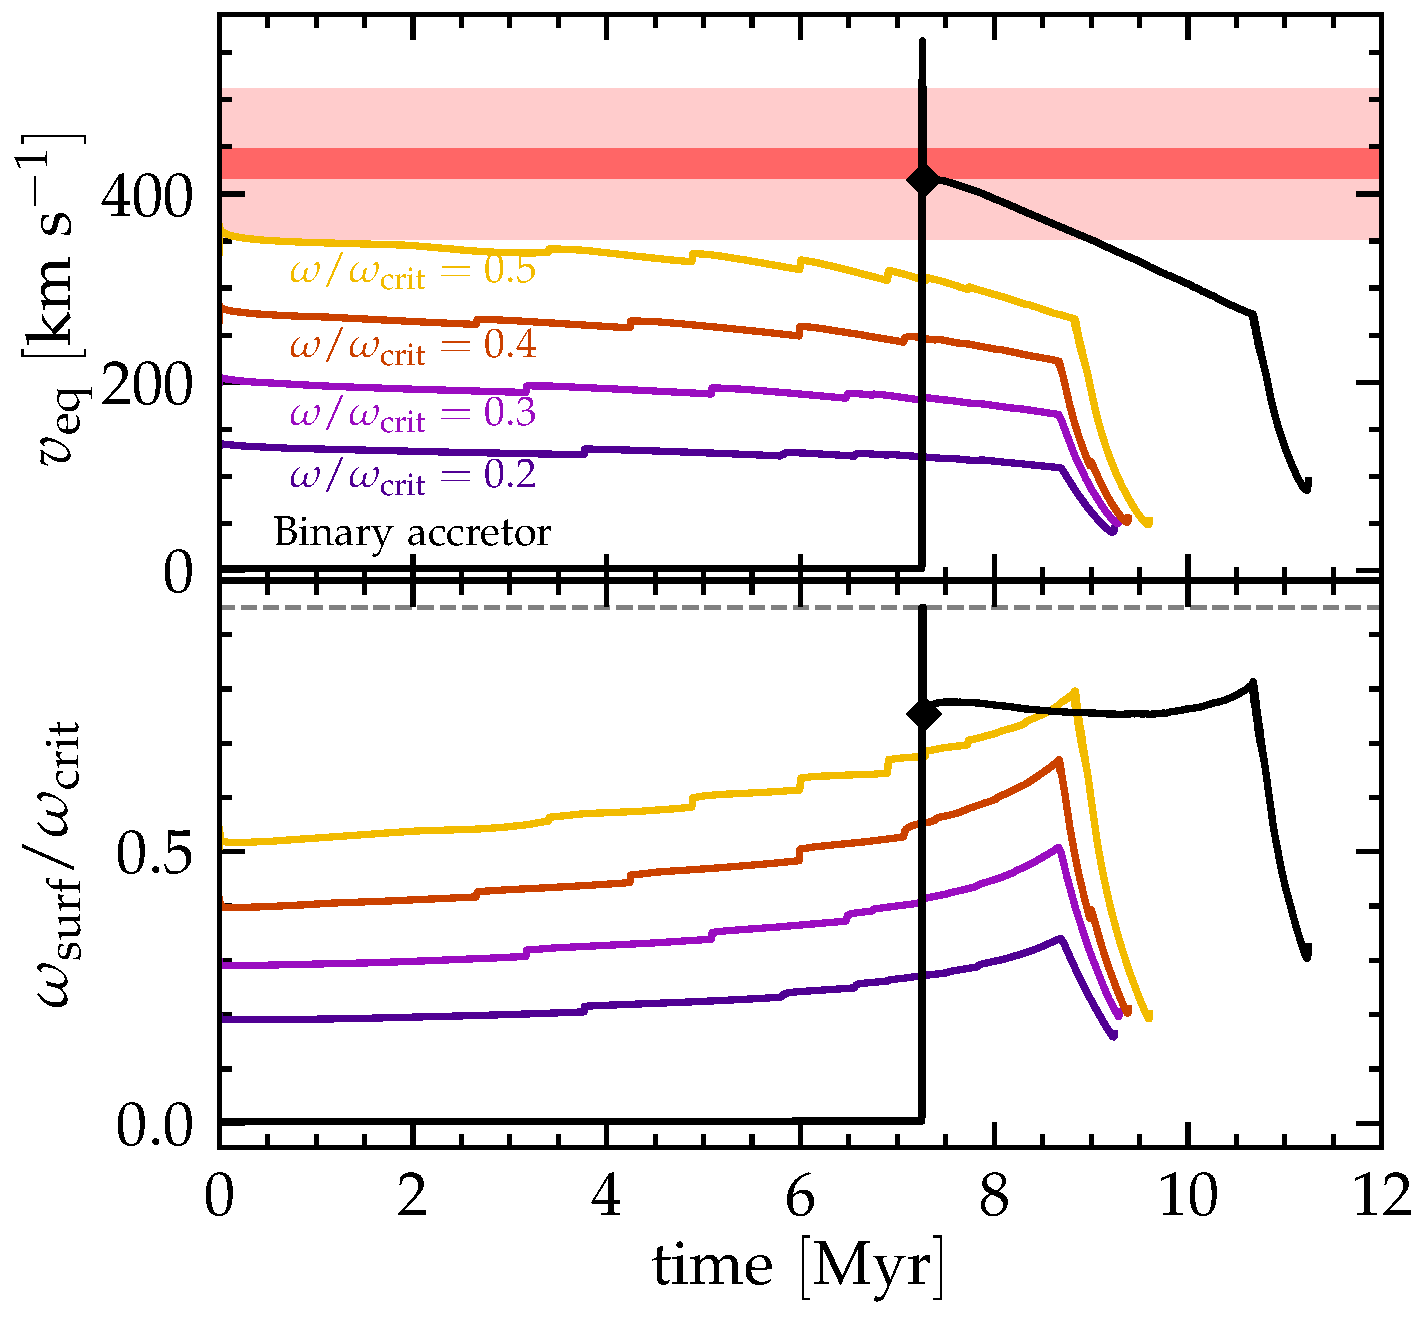
\includegraphics[width=0.5\textwidth]{zeta_rot}
  \caption{Surface averaged rotation rate for the accretor
    model. Shortly after $\sim$7\,Myr the mass transfer quickly spins
    up the accretor at critical rotation. By the time the donor
    detaches from the RLOF the accretor is still spinning at
    $\sim$$400\,\kms$. At this point (beginning of the dot-dashed line), we continue the evolution as a single star, and the accretor quickly spins down. Note however that we use a wind mass-loss rate from \cite{vink:01}, which is observed to be
    $\sim$2 orders of magnitude too high.}
  \label{fig:rot}
\end{figure}


\begin{figure}[htbp]
  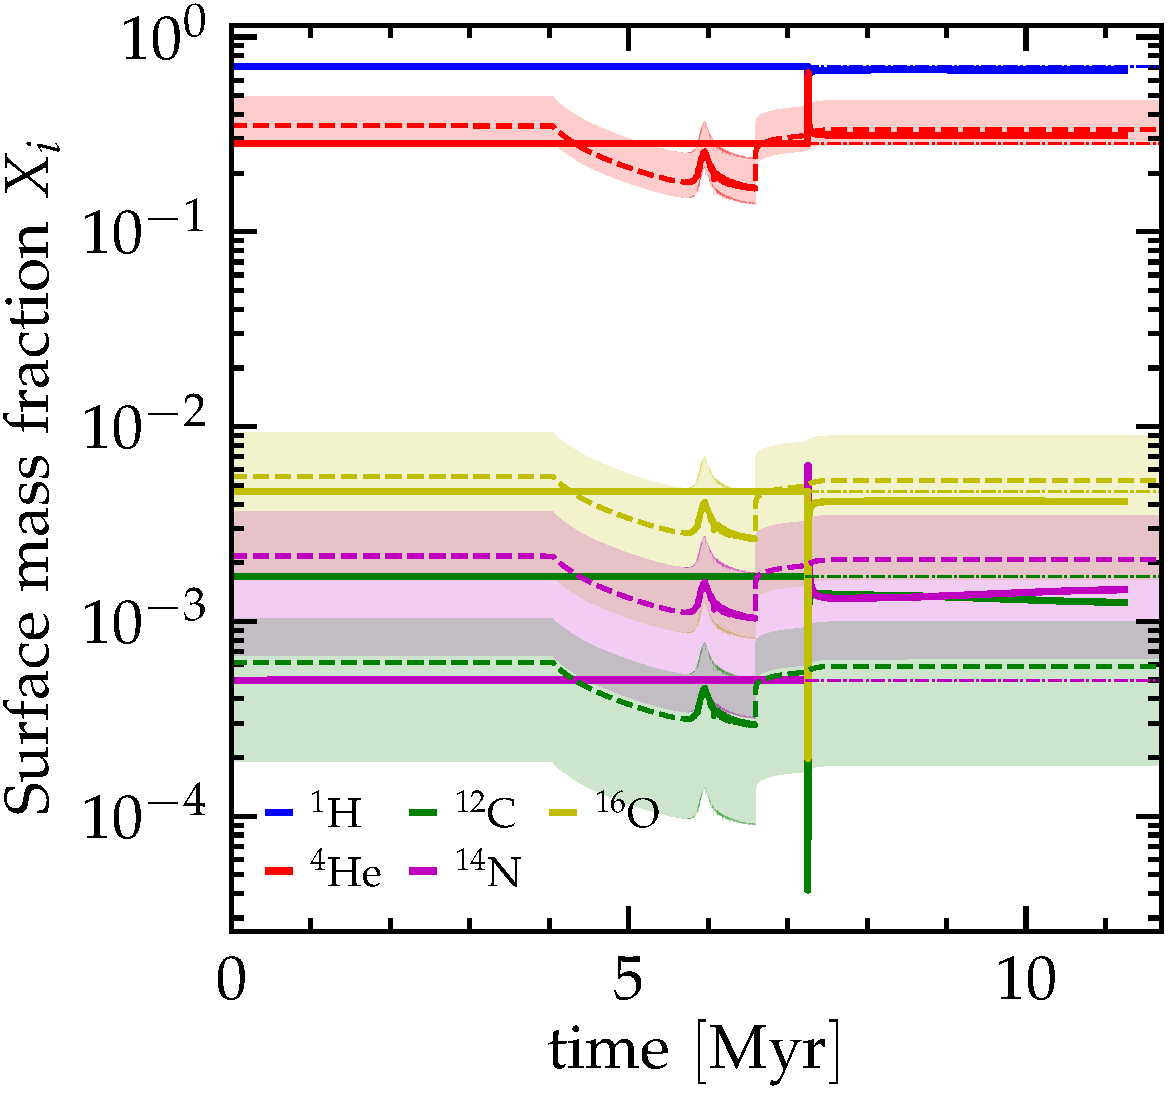
\includegraphics[width=0.5\textwidth]{composition_zeta}
  \caption{Evolution of the surface composition of the accretor. The
    thin dot-dashed lines show the initial mass fractions, the dashed
    line show the mass fractions from \cite{villamariz:05} with the
    corresponding shaded area for the errorbars. These evolve in time
    since we use the surface mass fraction of hydrogen to convert the
    reported number fractions into mass fraction. The solid lines show
    the surface mass fractions of the accretor, which deviate from the
    initial values during RLOF because of accretion, and afterwards
    because of internal mixing. }
  \label{fig:surface_ab}
\end{figure}

\section{Robustness of the model}
\label{sec:param_variations}
\todo{In this section we investigate the sensitivity of our results to
  physical parameters}

\todo{
  Binary parameters:
  \begin{itemize}
  \item $M_1$
  \item $M_2$
  \item $P$
  \item J-accretion
  \end{itemize}
}

\todo{
  Single star parameters:
  \begin{itemize}
  \item thermohaline mixing
  \item Eddington-Sweet circulations
  \item metallicity
  \end{itemize}
}

\todo{others?}

\section{Conclusions}
\label{sec:conclusions}


\software{
  \texttt{mesaPlot} \citep{mesaplot},
  \texttt{mesaSDK} \citep{mesasdk},
  \texttt{ipython/jupyter} \citep{ipython},
  \texttt{matplotlib} \citep{matplotlib},
  \texttt{NumPy} \citep{numpy},
  \MESA \citep{paxton:11,paxton:13,paxton:15,paxton:18,paxton:19}
}

\section*{Acknowledgements}



\appendix

\section{\texttt{MESA} setup}
\label{sec:software}

\todo{MLT--?}

\todo{possibly move to methods}
We use \code{MESA} version 15140 to compute our models.  The
\code{MESA} equation of state (EOS) is a blend of the OPAL \citet{Rogers2002}, SCVH
\citet{Saumon1995}, PTEH \citet{Pols1995}, HELM \citet{Timmes2000},
and PC \citet{Potekhin2010} EOSes. \todo{check if updated EOS?}

Radiative opacities are primarily from OPAL \citep{Iglesias1993,
  Iglesias1996}, with low-temperature data from \citet{Ferguson2005}
and the high-temperature, Compton-scattering dominated regime by
\citet{Buchler1976}. Electron conduction opacities are from
\citet{Cassisi2007}.

Nuclear reaction rates are a combination of rates from NACRE
\citep{Angulo1999}, JINA REACLIB \citep{Cyburt2010}, plus additional
tabulated weak reaction rates \citet{Fuller1985, Oda1994,
  Langanke2000}. Screening is included via the prescription of
\citet{Chugunov2007}.  Thermal neutrino loss rates are from
\citet{Itoh1996}. We use a
22-isotope nuclear network (\texttt{approx\_21\_plus\_cr56}).

We treat convection using the Ledoux criterion, and include
thermohaline mixing and semiconvection, both with an efficiency factor
of 1. We assume $\alpha_\mathrm{MLT}=1.5$ and use \todo{fix}
\cite{brott:11} overshooting for the convective core
burning. \todo{fix} Moreover, we employ the MLT++ artificial
enhancement of the convective flux \citep[e.g.,][]{paxton:15}. Stellar
winds are included using the algorithms from \cite{vink:01} with an
efficiency factor of
1.% and \cite{nugis:00} when the surface en abundance
% is below 0.4 and $T_\mathrm{eff}>10^{4.7}\,\mathrm{K}$. We use a
% hyperbolic tangent interpolation between the two for
% hydrogen-deficient surfaces with
% $10^{4.5}\,\mathrm{K}\leq T_\mathrm{eff}\leq10^{4.7}\,\mathrm{K}$. In
% both cases, we use an efficiency factor of 1, and our post-merger models never
% become cool enough to use a cool wind algorithm \citep[e.g.,][]{renzo:17}.

The inlists, processing scripts, and model output will be made available at~\href{link}{link}.

\bibliographystyle{aasjournal}
\bibliography{./zeta_ophiuchi.bib}

\end{document}

%%% Local Variables:
%%% mode: latex
%%% TeX-master: t
%%% End:
